\section{Sistema de Refrigeração}
O sistema de refrigeração é uma etapa crucial do projeto da transportadora de órgãos, atendendo ao requisitos definidos o recipiente em que o órgão é armazenado e transportado deve se manter refrigerado durante o período de transporte. Refrigeração pode ser definida como todo processo de remoção de calor, redução e manutenção de temperatura de um espaço ou material abaixo da temperatura ambiente (JÚNIOR, 2003). Portanto, a partir da análise das características da demanda de refrigeração e do conhecimento para a construção e integração do produto, foram levantadas duas opções de resfriamento:
	\begin{itemize}
		\item Refrigeração Termoelétrica - Células Peltier;
		\item Refrigeração por Compressão Mecânica de Vapor - Compressor.
	\end{itemize}
	
	O refrigerador termoelétrico utiliza-se de dois materiais distintos, como pares termoelétricos convencionais. Há duas junções entre esses dois materiais em um refrigerador termoelétrico, uma está localizada no espaço refrigerado e a outra no meio ambiente. Quando se aplica uma diferença de potencial, a temperatura da junção que se encontra no espaço refrigerado diminui e a temperatura da outra junção aumenta. Operando em regime permanente, ocorrerá uma transmissão de calor do espaço refrigerado para a junção fria. A outra junção se encontrará a uma temperatura acima à ambiente e haverá então uma transmissão de calor para o local.
	
	A utilização dos módulos de peltier tem as seguintes vantagens: 
	
	\begin{itemize}
		\item Ausência de peças móveis e  gases refrigerantes  para refrigeração; 
		\item Aquece e resfria dependendo apenas da polaridade da alimentação;
		\item Ausência de barulho e vibrações;
		\item Tecnologia 100 por cento estado sólido; 
		\item Tamanho da solução reduzido e alta durabilidade;
		\item Funcionam em qualquer orientação com / sem gravidade diferente dos refrigeradores baseados em compressores.
		
	\end{itemize}
	
	Já o sistema de refrigeração por compressão mecânica de vapor funciona simplificadamente da seguinte forma, o fluido refrigerante que percorre um circuito fechado para absorver e remover o calor de um espaço que necessita de arrefecimento. Em qualquer processo de refrigeração, ocorre a transferência de calor de um ambiente para outro com a ajuda de um agente externo, que no caso deste sistema é o compressor (FERRAZ, 2008).
	
	Ao se optar por este tipo de sistema de refrigeração, têm-se como vantagens:
	\begin{itemize}
		\item Baixo consumo;
		\item Maior eficiência.
	\end{itemize}

	Em um primeiro momento optou-se pela refrigeração termoelétrica, realizaram-se vários testes de configurações para a célula peltier, entretanto não obtivemos resultados satisfatórios com relação à temperatura atingida dentro da câmara a ser refrigerada, apesar de conseguirmos uma temperatura adequada na face da módulo termoelétrico. A figura abaixo apresenta alguns dos testes realizados.
	
	
	\begin{figure}[H]
		\begin{center}
			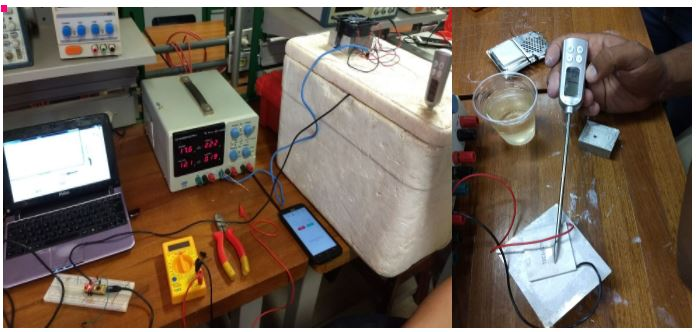
\includegraphics[scale = 0.8]{figuras/teste_Peltier.JPG}
			\caption{Testes iniciais utilizando a célula Peltier}
		\end{center}
	\end{figure}
	
	Devido aos resultados insatisfatórios, optou-se então pelo sistema por compressão mecânica de vapor, tendo como fonte de fornecimento uma bateria estacionária. O funcionamento do sistema de refrigeração construído está expresso na figura a seguir:
	\begin{figure}[H]
		\begin{center}
			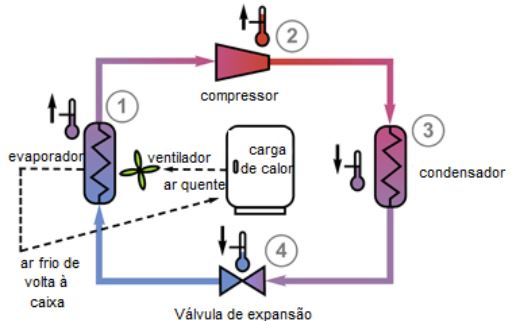
\includegraphics[scale = 0.75]{figuras/esquematico_compressor.JPG}
			\caption{Diagrama esquemático do sistema com compressor}
		\end{center}
	\end{figure}
	
	\subsection{Dimensionamento do Sistema}
		\subsubsection{Cálculo de Carga Térmica}
		Os cálculos da carga térmica objetivam determinar a quantidade de calor que deverá ser removida da caixa transportadora de órgãos, para que se atinja as condições adequadas para o armazenamento e transporte do órgão.
		
		Para desenvolver os cálculos da carga térmica do sistema, foram levantados os seguintes dados do sistema:
		\begin{enumerate}
			\item Dimensões da caixa interna (que contém o órgão):
				\begin{itemize}
					\item Altura: 0,2 m.
					\item Largura: 0,25 m.
					\item Profundidade: 0,25 m.
				\end{itemize}
			\item Dimensões da caixa externa:
				\begin{itemize}
					\item Altura: 0,3 m
					\item Largura: 0,3 m.
					\item Profundidade: 0,3 m.
				\end{itemize}
			\item Capacidade (volume) da caixa térmica: 0,0027 $m^3$ (27 L)
			\item Temperatura interna de operação: $2^oC$
			\item Temperatura externa à caixa:$ 35^oC$.
			\item Material de isolamento térmico: Poliestireno expandido.
			\item Espessura do material de isolamento térmico: 0,07 m.
			\item Tempo de resfriamento: 45 minutos.
		\end{enumerate}
		
		\subsubsection{Cálculo da energia e potência térmica do órgão:}
		Este cálculo se refere à quantidade de calor associada ao órgão e pode ser calculada pela equação:
		\begin{equation}
		Q = m \times c \times \Delta T
		\end{equation}
		
		Sendo: 
		$Q$ = energia térmica (KJ)
		
		$m$ = massa (g)
		
		$c$ = calor específico $(\frac{cal}{g^oC)}$
		
		$\Delta T$ = Variação da temperatura $(^oC)$
		
	Logo, a energia térmica do órgão é:
	$$
	Q_{órgão} = 13,8 KJ
	$$	
	
	Logo, a energia térmica do órgão é:
	$$
	P_{órgão} = \frac{13,8}{\Delta t} \approx 5,1 W
	$$
	
	\subsubsection{Cálculo da energia e potência térmica da embalagem com solução Viaspan na qual o órgão está contido}
	Aplicando a equação para a energia térmica, tem-se:
	$$
	Q = 500  \times 0,97 \times 33 \approx 67 KJ
	$$
	Aplicando a equação para a potência térmica, tem-se:
	$$
	P = \frac{67 KJ}{2700} \approx 24,8W
	$$
	
	\subsection{Cálculo da energia e potência térmica do alumínio da caixa interna}
	
	Aplicando a equação para a energia térmica, tem-se:
	$$
	Q_{aluminio} = 3000 \times 0,22 \times 33 \approx 91,2 KJ
	$$
	
	Aplicando a equação para a energia térmica, tem-se:
	$$
	P_{aluminio} \approx 33,8
	$$
	
		A soma das potências térmicas do órgão, da embalagem contendo a solução Viaspan e do alumínio fornecem a potência térmica total do interior da caixa, necessária ao resfriamento.
		
		A caixa externa também está envolvida nos cálculos de potência térmica devido a transferência de calor que ocorre entre a vizinhança e o sistema.
		
		\subsubsection{Cálculo da resistência térmica $(Rt)$ e o coeficiente global de transferência de calor (U)}
		
		A resistência térmica é calculada a partir da equação
		
		$$
		R_t = \frac{L_{isopor}}{K_{isopor}}
		$$
	
	Sendo:
	$R_t$ = resistência térmica $\frac{m^2K}{W}$
	
	L = espessura (m)
	
	K = condutibilidade térmica $\frac{W}{mK}$
	
	Aplicando a equação, tem-se:
	$$
	R_t = \frac{0,7}{0,007} \approx 2\frac{m^2K}{W}
	$$
	
	O coeficiente global de transferência de calor é calculado a partir da equação.
	\begin{equation}
	U = \frac{1}{R_t}
	\end{equation}
	Aplicando a equação acima, tem-se:
	$$
	U = 0,5 \frac{W}{m^2 K}
	$$
	
	A quantidade de calor que atravessa as paredes da caixa externa é dada pela equação a seguir:
	\begin{equation}
	Q = U \times A \times \Delta T
	\end{equation}
	
	Aplicando a equação, considerando-se a área total da caixa, tem-se:
	
	$$
	Q = 0,5 \times 0,54 \times 33K
	$$
	Por fim, a potência térmica total do sistema é calculada pela soma da potência térmica interna da caixa junto a quantidade de calor que atravessa as paredes da caixa externa.
	
	Desta forma, conclui-se que o sistema de refrigeração deve suprir a potência de 72,61 W para o resfriamento às condições desejadas.
	
	\subsection{Evaporador}
	Para determinar a área do trocador de calor, podemos utilizar o Método de  Média Logarítmica das Diferenças de Temperatura que é dado pela seguinte relação:
	
	\begin{equation}
	Q = k \times A \times \Delta T_{ln}
	\end{equation}
	
	Onde:
	
	Q - taxa de transferência térmica 
	
	K - coeficiente de transferência de calor global
	
	A - área de superfície de transferência de calor
	
	$\Delta T_{ln}$
	
	
Como o valor do coeficiente global de transferência de calor (K) pode variar, conforme a tabela abaixo,
	\begin{figure}[H]
	\begin{center}
	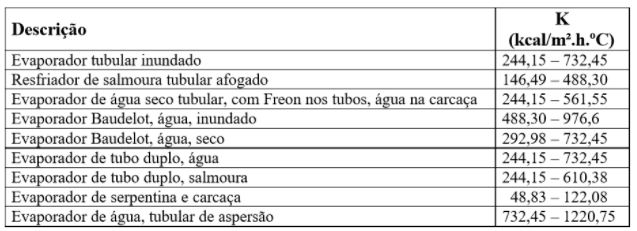
\includegraphics[scale =1]{figuras/Tabela_K}
	\caption{Tabela com os possíveis valores de K}
	\end{center}
	\end{figure}
	
	e considerando o pior dos casos de transferência de calor, obtemos um valor de 48,83 para um evaporador de serpentina e carcaça, que é o nosso caso.
	
	A capacidade frigorífica ($Q_0$) é a quantidade de calor por unidade de tempo retirada do meio que se quer resfriar (produto) através do evaporador do sistema frigorífico. Para o sistema operando em regime permanente desprezando-se a variação de energia e potencial, pela primeira lei da termodinâmica obtém-se: 
	
	\begin{equation}
	Q=m_f \times (h_1-h_4)
	\end{equation}

	\begin{figure}[H]
		\begin{center}
			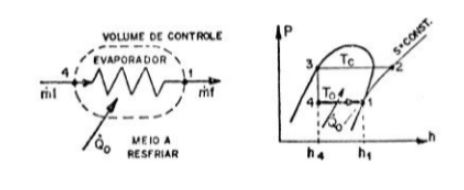
\includegraphics[scale =1]{figuras/Volume_Evaporador}
			\caption{Volume de controle aplicado ao evaporador e a indicação do processo }
		\end{center}
	\end{figure}
	
	$Q_0$ é a capacidade frigorífica  do ciclo operando em temperaturas $TC$ e $T_0$ para $m_f$, entalpia específica $h_1$ e  $h_4$. O fluxo de massa de refrigerante (mf) deve ser mantido pelo compressor. Normalmente se conhece a capacidade frigorífica que deve ter o sistema de refrigeração, que deve ser igualada à carga térmica, se estabelecermos o ciclo de refrigeração que deve operar o sistema podendo assim determinar o fluxo de massa e, consequentemente, o compressor necessário ao sistema (JÚNIOR, 2005).
	
	 A quantidade de calor retirado por um quilo de refrigerante através do evaporador é denominada “Efeito Frigorífico - E.F.”, isto é :
	 \begin{equation}
	 EF = h_1-h_4
	 \end{equation}
	 Então, substituindo pelos dados coletados:
	 
	 $$
	 m_f=9,81 \frac{Kg}{h}
	 $$
	 \subsection{Compressor}
	 Para o dimensionamento do compressor, é necessário calcular a potência necessária para fazer o fluido refrigerante circular pela serpentina. Essa potência foi encontrada a partir da formulação: 
	 
	 \begin{equation}
	 W_c = m_f \times (h_2 - h_1)
	 \end{equation}
	 
	 Sendo:
	$ W_c$ -  potência teórica do compressor); 
	
	 $m_f$ - fluxo de massa refrigerante;
	 
	 $h_2$ -  entalpia no início da compressão;
	 
	 $h_1$ - entalpia no final da compressão;
	 
	 \section{Estrutura do Conjunto de Refrigeração}
	 Após o dimensionamento do Sistema de Refrigeração, ocorreu a montagem do sistema final. O sistema dimensionado foi acoplado a estrutura geral do projeto, conforme demonstrado na Figura abaixo
	 	\begin{figure}[H]
	 		\begin{center}
	 			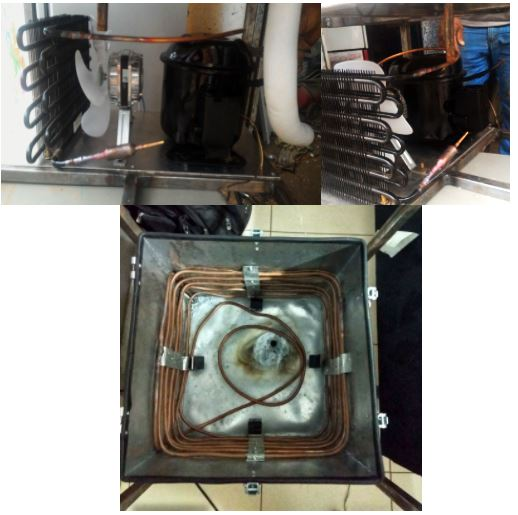
\includegraphics[scale =1]{figuras/Estrutura_refrigeracao}
	 			\caption{Estrutura do sistema de refrigeração }
	 		\end{center}
	 	\end{figure}
	 O compressor escolhido que satisfazia todas as necessidades dimensionadas, possui as seguintes especificações:
	 
	 	 	\begin{figure}[H]
	 	 		\begin{center}
	 	 			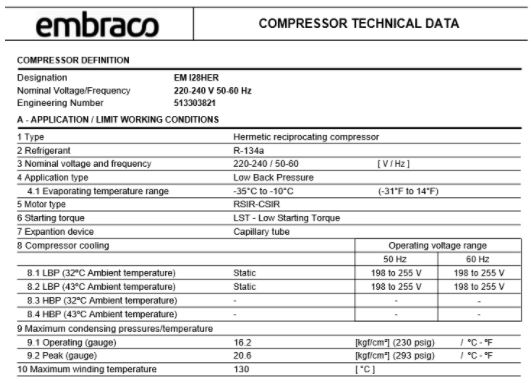
\includegraphics[scale =1]{figuras/caracteristicas}
	 	 			\caption{Especificações Técnicas do Compressor.
	 	 				 }
	 	 		\end{center}
	 	 	\end{figure}
	 	
\section{Sistema de Alimentação}
As fontes de energia que serão utilizadas para alimentar o produto, incluindo o sistema de refrigeração e os componentes elétricos e eletrônicos, são a rede elétrica comum brasileira e um banco de baterias. O banco de baterias será dimensionada a fim de manter os subsistemas em perfeita operação durante o período solicitado de 48 horas.

\subsection{Diagrama do Sistema}
A Figura a seguir apresenta o diagrama elétrico simplificado do produto. Ele representa o circuito de alimentação utilizado, desde a fonte de energia --- rede elétrica padrão --- até o uso final em seus componentes elétricos e eletrônicos.  É importante ressaltar que este diagrama será refinado ao longo dos pontos de controle, pois o  sistema pode ser retificado para melhor atender às condições de contorno que forem encontradas durante a execução do projeto.

\begin{figure}[H]
\begin{center}
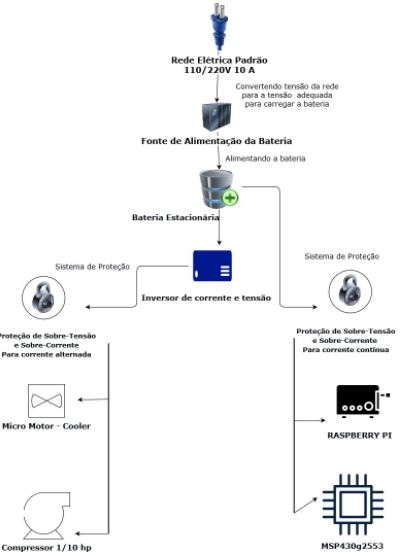
\includegraphics[scale = 1.2]{figuras/Diagrama_Simp.JPG}
\caption{ Diagrama Elétrico Preliminar}
\end{center}
\end{figure}

O sistema foi dimensionado com um fator de segurança elevado, pois a proposta de projeto é de um sistema de acondicionamento de órgãos para transplante. Sendo assim, o nível de confiabilidade do produto deve ser extremamente alto, para isso todo o sistema de alimentação foi dimensionado relacionando o sistema ao tempo de operação necessário ao transporte e diretamente ao consumo de energia advinda da bateria.


\subsection{Dimensionamento das Baterias}
	Baterias têm a finalidade de armazenar energia e liberá-la em determinada periodicidade, e de forma controlada. Sua escolha deve ser adequada às necessidades de consumo energético do projeto, e considera os dados de corrente elétrica e tensão. Para a seleção da bateria adequada deve-se estudar se ela é capaz de armazenar a energia total demandada às necessidades do projeto, e se ela consegue entregar toda a energia necessária ao funcionamento do equipamento. O processo de dimensionamento do banco de baterias deve ser realizado inicialmente e depois sucessivamente aperfeiçoado, em função dos demais dimensionamentos e ajustado em função dos custos, disponibilidade de mercado, entre outros.

	O processo de dimensionamento deve seguir algumas etapas, a primeira delas é definir o tipo de bateria a ser utilizado. Dentre as opções de bateria disponíveis no mercado, optou-se pela bateria estacionária. Sua vida útil é de aproximadamente 5 anos, devido à sua composição com materiais internos mais sobres se comparada às baterias automotivas, por exemplo. Podem, também, suportar descargas de até 80\% de sua capacidade, sem prejudicar sua vida útil, e resistem a ciclos de carga ou descarga mais profundos. Tais características proporcionam maior confiabilidade ao funcionamento do projeto pelo uso da bateria estacionaria.
	
	Após a escolha do tipo de bateria, deve ser analisada a profundidade de descarga com que se vai trabalhar. Quanto mais profundos os ciclos de descarga-carga, menor a vida útil da bateria. Ou seja, reduzir-se a capacidade da bateria, gasta-se menos no início, porém as baterias durarão menos e os gastos com reposição serão maiores. Um valor usado para essa profundidade de descarga para ciclos diários com baterias de chumbo-ácido é de 10\% a 20\%. Para ciclos esporádicos, podem ser utilizados ciclos mais profundos, da ordem de 60\%. 
	
	A capacidade do banco de baterias em Ah pode ser calculada conforme a expressão abaixo: 
	
	\begin{equation}
	Capacidade(Ah) = \frac{Consumo(\frac{Wh}{dia}) \times Autonomia(dias)}{V_{Baterias}(V)\times profundidade(pu)}
	\end{equation}

O dimensionamento da bateria requer inicialmente a relação de potência demandada para suprir as necessidades dos componentes elétricos do projeto, como mostra a tabela a seguir:

\begin{table}[H]
\caption{Consumo energético dos componentes}
\begin{tabular}{|p{4 cm} |c |c |c |}
 \hline
   \textbf{COMPONENTE} &\textbf{ALIMENTAÇÃO (V)}  &\textbf{CORRENTE (A)} & \textbf{POTÊNCIA (W)} \\
   \hline
  \textbf{MSP430g2553} &5 & 330$\mu$& 1,65 mW \\
   \hline
   \textbf{RASPBERRY PI}&5 &2,5 & 12,5 \\
   \hline
  \textbf{PROTETOR } &12 &26,5m &318m \\
   \hline
  \textbf{COMPRESSOR $\frac{1}{10}HP$} &12 & 2,4& 28,33 \\
   \hline
  \textbf{MICRO MOTOR} &12 &260,9m &3,6  \\
   \hline

\end{tabular}
\end{table}

Ao somar todas as cargas necessárias, o total foi de 229,819 Wh, já o consumo de corrente fica em 3,5365 A/h. O principal problema é o alto valor de partida do motor-compressor, o que é chamado de corrente de pico, no caso do motor-compressor utilizado, a corrente pode atingir um o valor entre 2-3 Ampères, o que requer atenção ao dimensionar a bateria para que ela suporte esse aumento inicial.


Com relação a profundidade da descarga no final da autonomia (pu) - utilizamos 0,6 (descargas mais profundas significam vida útil menor para a bateria e menos profundas um investimento inicial maior). Sendo que o consumo total é obtido a partir do levantamento das cargas, a autonomia de 5 horas.

Logo, 
$$
Capacidade \approx 33,2439 Ah
$$


\subsection{Dimensionamento do Inversor}
Inversores são conversores estáticos que, segundo Matakas Jr. E Komatsu (2011) transformam corrente ou tensão de forma contínua para a alternada. Muitos equipamentos operam em corrente/tensão contínua, sendo que a rede elétrica opera em corrente/tensão contínua. Portanto, a maneira mais simples de se trabalhar sem necessidade de mudanças drásticas em nenhum dos dois sistemas é se utilizar um inversor.

Este equipamento pode ser monofásico ou trifásico, sendo que o modelo utilizado no projeto será monofásico, e irá converter 12V da bateria que alimenta o sistema para 220V, valor de tensão que os outros componentes do sistema trabalham. Neste caso, com apenas duas chaves eletrônicas e uma fonte de tensão CC dividida é possível obter o inversor desejado.

Os inversores podem operar com duas tecnologias, senóide modificada ou senóide pura. No primeiro caso, formam uma onda quadrática, aproximando-se da senoidal AC, bom custo x benefício e pode ser aplicado na maioria dos casos, exceto para motores. O segundo caso pode ser usado como suprimento de energia AC em qualquer sistema, o que difere é o valor e o tamanho.

Um inversor bem dimensionado tem a potência maior que o consumo dos equipamentos para evitar que este trabalhe sempre em máxima potência,em suma um inversor é projetado em 3 estágios, oscilador, driver de corrente e transformador.
\begin{figure}[H]
	\begin{center}
		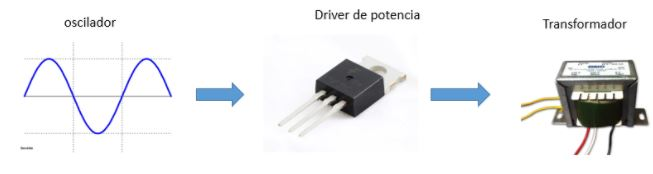
\includegraphics[scale = 0.75]{figuras/dim_inversor.JPG}
		\caption{ Diagrama Elétrico Preliminar}
	\end{center}
\end{figure}

Em primeiro lugar o oscilador transforma a corrente contínua em uma onda quadrada de 60Hz, que precisa ser adequada para uma onda senoidal, para isso é utilizado um filtro passa faixa centrado em 60Hz para eliminar as harmônicas indesejadas e obter uma onda senoidal mais eficaz possível. Entretanto, a saída do oscilador possui uma corrente muito baixa, por isso é necessário um ganho de corrente, para que seja entregue uma potência satisfatória na entrada do primário do transformador. Como a potência requerida é muito alta, se faz necessário que sejam inseridos vários transistores em paralelo para aumentar o ganho de corrente.

Na última fase o transformador faz a elevação da tensão para 220V que é a tensão necessária para ligar o compressor.

\subsection{Requisitos}
Com vistas à concepção e validação da solução, foram definidos os requisitos relativos ao subsistema de alimentação e refrigeração do produto:

\subsubsection{Requisitos Funcionais}
O sistema de alimentação deve ser capaz de:
\begin{itemize}
\item Armazenar energia elétrica;
 \item Fornecer energia para os componentes elétricos e eletrônicos de controle e monitoramento do produto;
 \item Fornecer energia para o sistema de refrigeração.
 \end{itemize}
\subsubsection{Requisitos Não Funcionais}
O sistema de alimentação deve ser capaz de:
\begin{itemize}
\item Prover a energia necessária para o bom funcionamento do produto durante um período máximo de 48 horas, com armazenamento de energia em baterias;
\item O sistema deve ser capaz de controlar a potência que será entregue as placas de peltier;
 \item Possuir eficiência energética aceitável, através de um controle de potência no sistema de refrigeração, escolha de componentes eletrônicos de baixa potência e sistemas de standby em determinados componentes não críticos do produto;
 \item Ser estável energeticamente, evitando picos de potência com componentes e segurança de circuitos.
 \end{itemize}